\chapter{Discussion and Recommendations}
\label{cha:disc-recomm}

In this chapter the achieved results are discussed, as well as some tasks that
have not been achieved. \Cref{cha:evaluation} already discussed how the final
product satisfied the client's requirements. This chapter goes more in-depth why
not all these requirements have been met.

Afterwards, some recommendations are made that will further enhance and provide
possible directions for future work on the product.

\section{Discussion}
\label{sec:discuss-discussion}

TODO: section introduction

\subsection{Language interpreters have to be on the classpath}
\label{sec:discuss-classpath}

\subsection{Textual representation of DynSem data types}
\label{sec:discuss-dynsem-string}


%\section{Eclipse Multithreading Issues}
\label{sec:eclipse-multithread}

The implementation of the Eclipse frontend has been a source of exposing many
shortcomings in the initial designs. These shortcomings and how they have been
resolved are discussed in this section.

\subsection{Single- versus multithreading}

The initial design assumed that the frontends and the backend would run in the
same thread. For a console based REPL, this assumption holds and greatly
simplifies the design. However, this assumption does not hold when the backend
has a frontend using a multithreaded GUI toolkit. This
assumption resulted in two problems, which are listed separately in the next
sections. The solution and changes made to the design are then discussed
afterwards.

\subsection{Blocking- versus non-blocking input}

In a multi-threaded environment, asking graphical text entry widgets for the
entered text is rarely a blocking process. The REPL backend at the time,
however, assumed that getting the user's input was always a blocking operation.
Therefore, when a conceptual Eclipse frontend was made, the REPL spun into an
infinite loop trying to execute empty expressions.

\subsection{Evaluating on the UI thread}

As explained in \cref{ssec:eclipse-plugin}, multi-threaded graphical user
interface toolkits often use multiple threads. One of these threads is
designated the ``UI thread'', or user interface thread. This thread is
responsible for processing events (such as mouse clicks) and updating the
graphical representation of the widgets. All tasks that perform long running
calculations are supposed to be run in a background thread, such that the UI
thread is free to process incoming events. Instead, if a long running
computation is run in the UI thread, the widgets on the screen stop responding
to the user and the program appears to be in a frozen state. This is exactly
what happened when the backend assumed to be run in the same thread as the
frontend: whilst the backend was evaluation expressions, Eclipse appeared to be
frozen due to this evaluation taking place in the UI thread from which the
execution was started. This issue would be worse in case blocking input
were to be used.

\subsection{Accustoming to multi-threaded frontends}

As indicated in the previous sections, the only solution to these problems is to
allow multi-threaded frontends. This meant that the assumption of every
operation running in the same thread no longer held. As a result, several
changes had to be made:

\begin{enumerate}
  \item Initially, a \texttt{``Repl''} class was present in the backend to
  centralize a REPL implementation. This class made too many assumptions on
  behalf of the frontends, among which blocking user input and the entire main
  loop of a REPL. The alternative is the \texttt{``IRepl''} interface (see
  \cref{sec:overview}), which defines the only method each frontend has in
  common: the \texttt{eval} method to evaluate input. It is now entirely up to
  the frontend on how to implement the read, print and loop steps, allowing for
  much more freedom.
  \item	The initial design provided ``hooks'' to the frontend to process results or
  errors. A frontend would register itself to process certain hooks, after which
  the registered method would be called. The registered methods would be called
  immediately after the evaluation was done, and on the same thread. In the
  conceptual Eclipse frontend, these hooks updated the widgets running in the UI
  thread. This then led to widgets being updated from a thread other than the UI
  thread. The solution, discussed in \cref{sec:visitor}, was to return the
  result to the frontend, allowing it to process the result whenever and however
  it needs.
\end{enumerate}

Not only did these changes resolve the threading issues, they also made for a
cleaner architecture overall. An additional advantage is that a much wider scala
of possible frontends is now supported.

%%% Local Variables:
%%% mode: latex
%%% TeX-master: "../main"
%%% End:


\section{Recommendations}
\label{sec:discuss-future}

This section makes several recommendations to the client for future work on the
delivered product. These recommendations come forth from requirements that have
not been implemented (see \cref{ssec:eval-requirements}) and opportunities for
improvements in the delivered product. First, recommendations are made to
improve the extend the REPL backend itself. Secondly, suggestions are made on
how to improve the Eclipse frontend. Finally, recommendations to provide
additional frontend implementations are made.

\subsection{Extending the functionality of the REPL}
\label{ssec:impr-backend}

TODO: introduction

\section{Read-Eval-Print Loops}
\label{sec:repl}

Many programming languages come with an interactive environment. This
interactive environment is an interface to the programming language's execution
engine. One common form of such an environment is an interface in which
expressions in a programming language are typed by the user, after which the
results of that expression are printed back to the user. Such an environment is
called a Read-Eval-Print Loop (REPL), although many different names are known,
including but not limited to \emph{language shell},
\emph{command-line interpreter} or \emph{interactive interpreter}. There
are subtle differences between these names and the name REPL. These are,
however, mostly of semantic value. In this report the term REPL is chosen,
because it conveys the notion of such an interactive environment well.

\subsection{Origin of REPLs}
\label{ssec:repl-origin}

The Lisp programming language is one of the first programming languages offering
such an interactive environment~\cite{Noyes92}. The name REPL comes from the
Lisp functions that implement it:

\begin{enumerate}
  \item The \texttt{read} function takes a user's input, which often is just one
    or several expressions as opposed to a complete compilation unit. It then
    parses this input and creates an AST.
  \item The AST created in the previous step is then passed on to the
    \texttt{eval} function, which evaluates it.
  \item The result yielded by the previous function is then printed out to the
    user by the \texttt{print} function.
  \item After having printed the result, the environment needs to \texttt{loop}
    back to the read state.
\end{enumerate}

Assuming the individual functions listed previously exist, a REPL can be created
in a single line of code simply by combining the functions:

\begin{lstlisting}[language=lisp]
(loop (print (eval (read))))
\end{lstlisting}

Lisp has a property called ``homoiconicity'': Lisp's syntax is similar to
its internal representation, resulting in the ability to infer a program's or
data object's state simply by reading its textual representation. Syntax and AST
are thus isomorphic, allowing data and code to be accessed and transformed
interchangeably.

In Lisp REPLs, therefore, arbitrary data objects yielded from a previous
expression can be used directly as input to the next expression. In programming
languages that do not belong to the Lisp family, homoiconicity is an unusual
feature. Interactive environments for these languages therefore often require
additional steps to read and evaluate expressions. This is part of the semantic
differences between the different names as mentioned in the introduction

\subsection{Advantages of REPLs}
\label{ssec:repl-advantages}

REPLs provide the ability to program interactively. Programming interactively
has multiple advantages.

When creating software solutions for an as of yet not well understood domain, it
is often not clear which data structures and algorithms are required. In such
cases, interactively developing and debugging software is an advantage over the
(oftentimes much slower) edit-compile-run-debug development style. This kind of
programming is called exploratory programming~\cite{Fritzson86}. Related to this
kind of exploration, programming interactively also provides a means for rapid
prototyping and bottom up programming~\cite{Graham93}.

The explorative and interactive features of a REPL also make it an excellent
tool for programmers to learn a new programming language. REPLs are also
combined with what is called literate programming to offer notebooks or language
playgrounds, as discussed in \cref{sec:literate-programming}.

\subsection{Execution Model}
\label{ssec:execution-model}

Every programming language defines an execution model, which specifies how
programs written in that language are executed. Among others, it specifies what
an indivisible unit of work is (a \emph{compilation unit}) and in what order
these units are executed. The implementation of an execution model is a compiler
and/or an interpreter. The execution model of a REPL shown in
\cref{fig:execution-model-repl} has a couple of differences with respect to that
of an interpreter or compiler.

One difference is what is considered an indivisible unit of work: a REPL might
accept singular expressions that a regular interpreter or compiler might
not. Usually the program is executed as a whole, without the need for smaller
blocks of execution. In contrast, when using a REPL, it might be desirable to be
able to execute say only a single statement as one unit of execution. The AST
output of the parsing step, as shown in \cref{fig:execution-model-repl}, can
therefore be a smaller unit than an AST found in the ordinary execution model.

Another difference between a compiler or an interpreter and a REPL is that a
REPL needs to dynamically maintain an environment such that each new expression
can be analyzed and evaluated within the environment of previously executed
expressions. For every expression entered, it thus needs to apply the outlined
steps again and update the environment it maintains in memory with the new
results. This could result in a different order of evaluation than when say an
interpreter executes a program as a whole.

\begin{figure}[t]
  \centering
  \includegraphics[width=\textwidth]{execution-model-repl}
  \caption{The execution model as shown in \cref{fig:spoofax-relations}, adapted
    for a REPL. The analysis and evaluation is done within the incrementally
    built environment of previously executed expressions.}
  \label{fig:execution-model-repl}
\end{figure}

\subsection{Functionality}
\label{ssec:repl-functionality}

Every REPL provided with a programming language has its own set of
functionality. However, a core set of functionalities, shared between all REPL
implementations, can be identified. To reach this core set of features,
well-known REPLs have been investigated and their features have been compiled
into a matrix as seen in \cref{table:feature-matrix}. These features are shortly
discussed below.

\begin{table}[]
\centering
\begin{tabular}{lccccccccc}
                                  & \rot{Python} & \rot{R} & \rot{\shortstack[c]{Common\\Lisp}} & \rot{\shortstack[c]{Haskell\\(GHCi)}} & \rot{Swift} \\
\toprule
Executes single expressions       & \cmark       & \cmark  & \cmark                             & \cmark                                & \cmark      \\
Executes statements               & \cmark       & \cmark  & \cmark                             & \cmark                                & \cmark      \\
Input history                     & \cmark       & \cmark  & \cmark                             & \cmark                                & \cmark      \\
Automatic binding of previously yielded values & \xmark & \xmark & N/A                          & \xmark                                & \cmark      \\
Persistent input history          & \cmark       & \cmark  & \xmark                             & \cmark                                & \cmark      \\
Multiline input editing           & \cmark       & \cmark  & \cmark                             & \cmark                                & \cmark      \\
Redefining identifiers            & \cmark       & \cmark  & N/A                                & \cmark                                & \cmark      \\
Error reporting                   & \cmark       & \cmark  & \cmark                             & \cmark                                & \cmark      \\
Semantic code completion          & \cmark       & \xmark  & N/A                                & \xmark                                & \cmark      \\
Help or documentation system      & \cmark       & \cmark  & \cmark                             & \xmark                                & \xmark      \\
Additional commands to the REPL   & \xmark       & \xmark  & \cmark                             & \cmark                                & \cmark      \\
Nested REPLs to enable debugging  & \xmark       & \xmark  & \cmark                             & \xmark                                & \xmark      \\
\bottomrule
\end{tabular}
\caption{A feature comparison of several well-known REPLs}
\label{table:feature-matrix}
\end{table}

\paragraph{Input history} REPLs keep a history of inputs, such that previously
entered expressions can be retrieved.

\paragraph{Automatic binding of previously yielded values} When an expression
has been evaluated, the yielded result is bound to an automatically created
identifier, such that it can be reused easily in future expressions.

\paragraph{Persistent history} The input history as discussed previously can be
recorded into a file (either per-project or globally) to enable a persistent
history of input.

\paragraph{Multiline input editing} Some constructs in a programming language
naturally span multiple lines. REPLs therefore provide multiline input editors
that recognise incomplete code and promptly switch to a multiline environment
when required.

\paragraph{Redefining identifiers} When using a REPL in an exploratory manner,
it is not uncommon to want to redefine an identifier's type or to completely
reimplement a method. In this way, a REPL can be different than its host
language, especially if the host language is a functional language that does not
allow variables' values to change once initiated.

\paragraph{Error reporting} A REPL typically has the same error reporting
functionality as an interpreter or a compiler, meaning it prints the error
message accompanied by the corresponding section of the source code.

\paragraph{Semantic code completion} Semantic code completion is a helpful tool
to provide an overview of the often many APIs a developer works with, adding to
the explorative nature of a REPL. Note that this is a restriction of syntactic
completion, which is offered by all the studied REPLs.

\paragraph{Help or documentation system} The exploratory nature of a REPL means
that one will often see new methods. Some REPLs (most notably Python's REPL with
Python's docstrings) offer a documentation system, so that the developer does
not have to exit the REPL to look up documentation.

\paragraph{Additional commands to the REPL} Some REPLs offer additional commands
to inspect the environment or to control their behavior. These commands are
oftentimes not in the syntax of the host language and are highly diverse between
REPL implementations. A notable example of a REPL offering such commands is
Haskell's GHCi~\cite{GHCi-commands}.

\paragraph{Nested REPLs to enable debugging} A notable feature of (mostly) Lisp
REPLs is that in case of an error, a new REPL is spawned inside the context of
this error. This REPL then has additional commands (see the previous feature) to
enable debugging and inspection of the error state. When the user has
resolved the error, the nested REPL exits and the user is returned to the
parent REPL. This can go to arbitrary depths.

%%% Local Variables:
%%% mode: latex
%%% TeX-master: "../main"
%%% End:


\subsubsection{Adding support for alternative evaluation strategies}
\label{ssec:discuss-alternate-eval}

As discussed in \cref{sec:eval-strat}, languages developed with Spoofax are not
limited to a single interpreter. Instead, there can be different strategies for
evaluation. While this has been taken into account for the design of the
product, only a DynSem evaluation strategy has actually been implemented.

Languages with a Java backend (such as IceDust%
\footnote{https://github.com/MetaBorgCube/IceDust}) therefore do not currently
work with the REPL. To add support for specific interpreters, a language should
provide the REPL with a named implementation of the
\texttt{``IEvaluationStrategy''}. The language designer can register alternative
evaluation strategies with the REPL by extending the Guice module of the backend
and overriding the \texttt{bindEvalStrategies} method.

Finally, the evaluation strategy that will be used to evaluate input terms can
be configured via the ShellFacet ESV extensions (see \cref{sec:esv-extensions})
as illustrated in \cref{lst:eval-method}.

\begin{lstlisting}[language=esv,caption={Setting the evaluation strategy.},label={lst:eval-method}]
module editor/SL-Shell

shell
    evaluation method : "dynsem"
\end{lstlisting}



\subsection{Improvements to the Eclipse frontend}
\label{ssec:impr-eclipse}

\input{discuss-recommend/eclise}

\subsection{Alternative Frontend Implementations}
\label{ssec:discuss-alternative-frontend}

\Cref{sec:frontends} showed that implementing different frontends is
straightforward: only a handful of interfaces have to be implemented in order to
provide a basic frontend. The client has expressed their interest in numerous
other frontends, which have not been implemented due to time contraints.
However, because providing additional implementations is straightforward,
several recommendations for additional frontends are made in this subsection.

\subsubsection{An IntelliJ Frontend}
\label{ssec:intellij}

As has been said before, an effort is currently underway to provide different
IDE-implementations of Spoofax. The Spoofax for IntelliJ IDEA
project\footnote{See:
\url{http://metaborg.org/en/latest/source/langdev/manual/env/intellij/}}
provides a plugin for the IntelliJ IDEA IDE. The client has expressed their
interest in having the REPL available in this IDE as well.

This IntelliJ IDEA REPL would then provide the same features as the current
console- and Eclipse REPLs.

%%% Local Variables:
%%% mode: latex
%%% TeX-master: "../main"
%%% End:


\section{Literate Programming}
\label{sec:literate-programming}

Just as with REPLs, the concept of literate programming is implemented in
various forms under various names. Therefore, this section starts with an
explanation of what literate programming is based on a few implementations.
Afterwards, the IPython implemention of literate programming is explored in more
detail.

Literate programming, as defined by Donald Knuth~\cite{knuth1984}, introduces
the ability to annotate source code with natural language. According to Knuth,
better documentation of programs is essential to make further progress in the
state of the art of programming.  To achieve this he proposes to write programs
not with the intention to explain the computer what to do, but with the
intention to explain to humans what the programmer wants a computer to
do~\cite{knuth1984} by mixing documentation and source code in a single file.
This idea of literate programming was realized in its original form as the
``WEB'' language developed during Knuth's research at Stanford University.

Even though the idea was conceived over thirty years ago, implementations are not
very common. However, in recent years the idea seems to gain popularity again.
A very recent implementation of literate programming is Apple's Swift
playgrounds~\cite{swift-playgrounds}. Swift playgrounds are interactive
documents or ``notebooks'' in which code is executed as it is typed, in
contrast to the non-interactive style of the ``WEB'' language in which \TeX{} and
PASCAL were combined into one language: \TeX{} served to document the program
and PASCAL to produce a machine-executable program.

In recent years, there has also been a particular focus on reproducible
research. While literate programming primarily aims to add documentation to
code, reproducible research focuses on adding code to documentation. More
specifically, reproducible research refers to the idea that scientific papers
should be augmented with the computer code used to carry out the
research~\cite{schulte2012}. Examples of recent projects claiming to support
both reproducible research and literate programming include the IPython
project~\cite{ipython2007} and Emacs Org-mode~\cite{schulte2012}.

\subsubsection{IPython with Jupyter notebooks}

IPython, together with Jupyter notebooks,
supports both reproducible research and literate programming. IPython was
partially inspired by other scientific tools already offering notebook-like
functionality, such as Matlab or Mathematica. Since its inception, the project
has been split off into IPython, which provides an interactive REPL and a
kernel that runs the user's code, and Jupyter notebooks, which provide the
notebook format and web application. Like Swift playgrounds, Jupyter notebooks
allow for REPL-style interactive editing; documentation and code can be edited
live and blocks of code can be reevaluated, printing their updated results.
Jupyter notebooks also allow for more complex graphical elements such as
3D-plots. See \cref{fig:ipython} for an example of an IPython notebook.

\begin{figure}[htb]
  \centering
  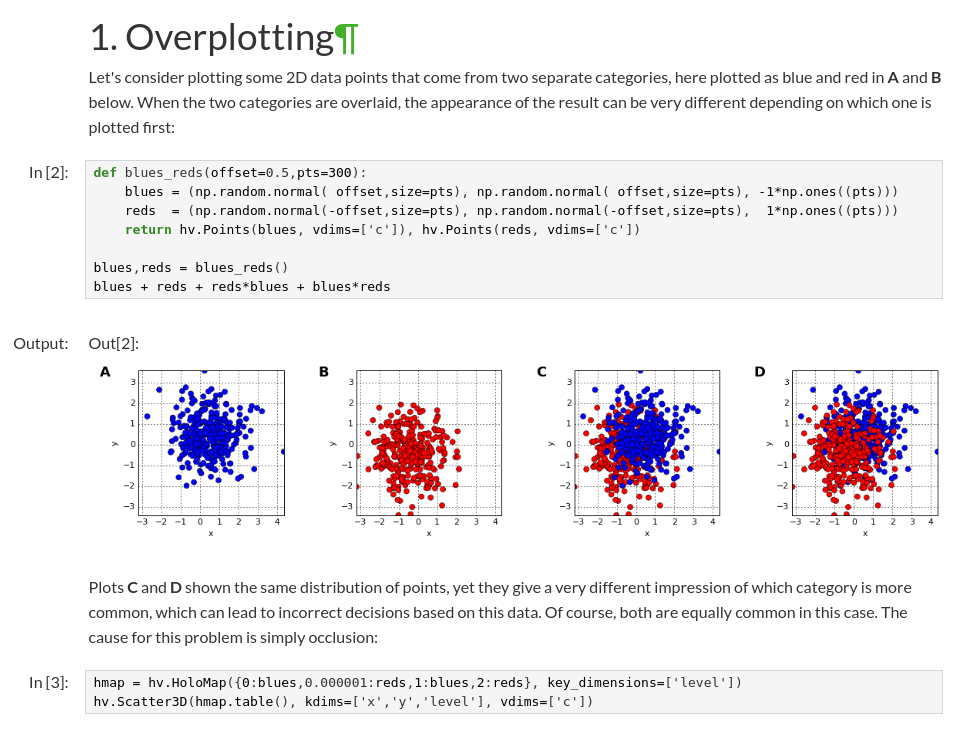
\includegraphics[width=\textwidth]{ipython}
  \caption{A plot from data in an IPython notebook.}
  \label{fig:ipython}
\end{figure}

As explained, IPython and Jupyter notebooks have become more or less separate
projects, to the extent that Jupyter notebooks can use several kernels.
Nowadays there are kernels for over forty languages that can be used in these
notebooks. This illustrates that in Python's case literate programming is more
or less an extension to the interactive IPython REPL. Since Jupyter notebooks
reuse the IPython REPL, the execution model used for Jupyter notebooks is
essentially the same as it is for IPython~\cite{ipython-execution}.

%%% Local Variables:
%%% mode: latex
%%% TeX-master: "../main"
%%% End:


%%% Local Variables:
%%% mode: latex
%%% TeX-master: "main"
%%% End:
